
The developed applications are divided into two distinct groups: the Client Side Application (CSA), or the User Interface,
and the Server Side Application , or the flight data/optimization API.
Both applications run independently from one another, although the CSA is dependent of the API,
and must communicate with it as to obtain solutions to the user requests.
Figure \ref{fig:system_architecture} introduces the architecture of the system,
aswell as the technologies on which the system relies, which will be adressed in the rest of this section. 


\begin{figure}[H]
  \centering
  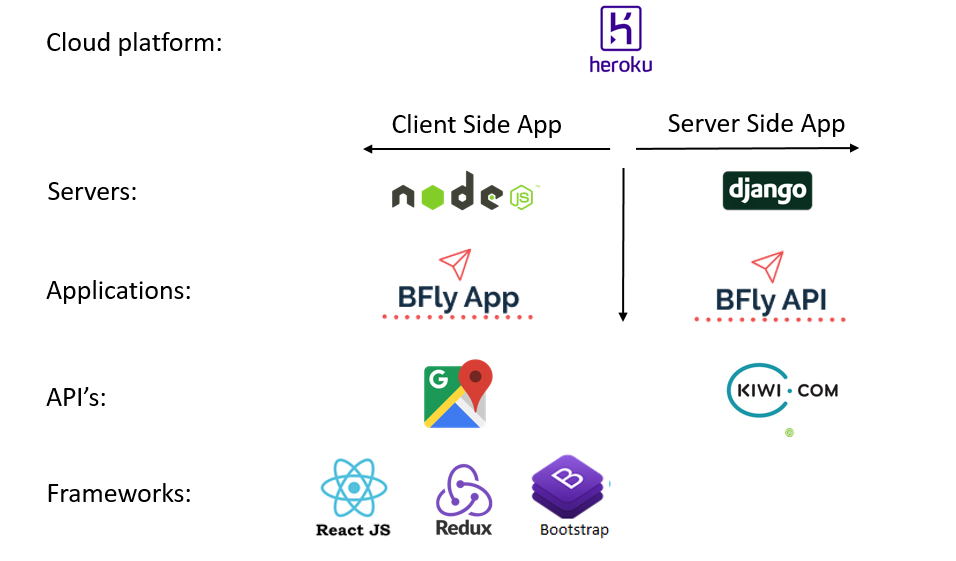
\includegraphics[width=\textwidth]{Figures/system_implementation/system_architecture_implementation.png}
  \caption{Architecture of the application.}
  \label{fig:system_architecture}  
\end{figure}


% The developed applications both run on \textit{Heroku}, a Cloud Platform as a service, 
% which, upon request, creates two separate servers, one for each application.
% The Client Side Application runs a \textit{Node.Js} server, which creates a 
% bundle file, that is served to the user, and contains all the necessary information to render the UI, handle the user input logic,
% and interact with the API. 
% In its turn, the API runs on \textit{Django}, which interacts with the webserver to read the user request, 
% and may execute particular instructions according to the selected route.

The developed applications both run on \textit{Heroku}, a Cloud Platform as a service, 
which, upon request, creates two separate servers, one for each application. 
These two servers are created by two different Web frameworks, namely Django for the server side app,
and Node for the client side. This means that using these frameworks, many of the low-level
implementation details associated to web development, as protocol details, sockets or thread management,
are handled directly by the respective framework \cite{python_wiki}, freeing the developer to actually work on the development 
of the application.